\newpage
\section{Funktionsmuster}
In diesem Abschnitt werden für gewisse Teilfunktionen des Roboters Funktionsmuster oder Prototypen erstellt. Damit können die Bewegungsabläufe und die technische Machbarkeit veranschaulicht werden. Ebenfalls können Probleme frühzeitig identifiziert und behoben werden.
\subsection{Piktogrammerkennung mit CNN}
\label{piktogrammerkennungMitCNN}
Das Ziel dieses Funktionsmusters ist es in erster Linie, Erfahrung zu sammeln mit OpenCV und der Piktogrammerkennung mit einem Convolutional Neural Network (CNN). Als CNN wurde eine vereinfachte Version der VGGNet Architektur gewählt.
Der Programmcode der Pythonscripts ist auf Github\footnote{https://github.com/randombenj/hslu-pren1/tree/master/pictogram\_detection} wie auch in Anhang zu finden.

\subsubsection{Trainingsdaten}
\image
   {img/piktogrammerkennung/collage.png}
   {Eine Bildmontage des multi-class deep learning dataset.}
   
Das Datenset besteht aus 500 Bildern über fünf Kategorien.
\begin{itemize}
    \item Hammer Piktogramm (100 Bilder)
    \item Farbkessel Piktogramm (100 Bilder)
    \item Lineal Piktogramm (100 Bilder)
    \item Bliestift Piktogramm (100 Bilder)
    \item Taco Piktogramm (100 Bilder)
 \end{itemize}
 
Die Trainingsdaten sind auf die Bilder in der Aufgabenstellung beschränkt. Um das Datenset zu vergrössern wurden aus den original Piktogrammen mithilfe von Dataaugmentation viele leicht abgeänderte Versionen erstellt. Das Ziel dieses CNN ist, dass es anhand dieser Trainingsdaten die Piktogramme in der realen Welt korrekt klassifizieren kann.

\subsubsection{Trainingsergebnisse}
Wie im Plot ersichtlich, wurde das CNN über 100 Epochs traniert und erreichte:
\begin{itemize}
    \item 99.9\% multi-label Klassifikationsgenauigkeit mit den Trainingsdaten (train\_acc)
    \item 98.9\% multi-label Klassifikationsgenauigkeit mit den Testdaten (val\_acc)
 \end{itemize}
 \image
   {img/piktogrammerkennung/trainingsergebnisse_piktogram.png}
   {Trainingsergebnisse des Funktionsmusters Piktogrammerkennung}
   
\subsubsection{Tests}
Um die Effektivität des Trainings zu testen wurden verschiedenen Testbilder dem CNN übergeben. Das Diagramm kann die Originalbilder mit weissem Hintergrund voneinander unterscheiden. Jedoch sobald sich eine Umgebung im Hintergrund des Bildes befindet, werden die Klassifizierungen sehr unpräzise.
\image
   {img/piktogrammerkennung/classifiedHammer.png}
   {Ergebnisse der Hammerklassifizierung}
   
\image
   {img/piktogrammerkennung/classifiedBucket.png}
   {Ergebnisse der Farbkesselklassifizierung}
   
\image
   {img/piktogrammerkennung/classifiedRuler.png}
   {Ergebnisse der Linealklassifizierung}
   
\image
   {img/piktogrammerkennung/classifiedPen.png}
   {Ergebnisse der Bleistiftklassifizierung}
   
\image
   {img/piktogrammerkennung/classifiedTaco.png}
   {Ergebnisse der Tacoklassifizierung}

\image
   {img/piktogrammerkennung/classifiedBucketBG.png}
   {Ergebnisse der Farbkesselklassifizierung mit Hintergrundumgebung}
   
\image
   {img/piktogrammerkennung/notClassifiedBucketBG.png}
   {Ergebnisse der Farbkesselklassifizierung mit viel Hintergrundumgebung}

\subsubsection{Fazit}
Dieses Funktionsmuster hat gezeigt, dass die Piktogramme bereits mit wenigen und simplen Testdaten mit einer sehr hohen Wahrscheinlichkeit korrekt klassifiziert werden. Vorausgesetzt, die Piktogramme sind mit schwarz auf weissem Hintergrund abgebildet und es befindet sich nichts weiter im Hintergrund. Der Ansatz, die Piktogramme mithilfe eines CNN mit einer vereinfachten VGGNet-Architektur zu erkennen, könnte also weiter verfolgt werden.  

Da die Piktogramme in der Realität jedoch nicht einfach schwarz auf weiss und ohne Hintergrundumgebung vorzufinden sind, könnte man für eine korrekt Identifizierung folgende Ansätze weiterverfolgen:
\begin{itemize}
    \item Mehr Trainingsdaten
    \item Breiter diversivizierte Trainingsdaten (z.B. mit passendem Hintergrund)
    \item Input an den Traingsdaten anpassen durch Herausfiltern der Region of interest (ROI)
    \item Anderes deep learning Modell verwenden
 \end{itemize}
 
Jedoch hat sich im Daily-Standup mit dem Coach herausgestellt, dass machine learning nicht der richtige Lösungsansatz für die endliche Problemstellung der Piktogrammerkennung ist! 

Da man lediglich fünf, bereits im Vorfeld bekannte Piktogramme erkennen muss, kann man das mit sogenanntem Template Matching\footnote{https://docs.opencv.org/master/d4/dc6/tutorial\_py\_template\_matching.html} realisieren. Hierbei werden Inputdaten mit den verschiedenen Templates, in unserem Fall die fünf Piktogramme, abgeglichen. Dabei wird versucht die verschiedenen Templates in den Inputdaten zu erkennen. 


\subsection{Hindernisserkennung}

Um die Treppe besteigen zu können, und nicht in die Hindernisse hineinzufahren, müssen
diese zuerst erkannt werden. Wie bereits bei anderen Kompenenten wird auch hier versucht, so einfach wie möglich zu bleiben.
Als erstes wird evaluiert, wie gut die Hindernisse mit einer Kamera
und simpler Bildverarbeitung, beispielsweise mittels OpenCV\footnote{https://opencv.org/}, erkannt werden
können.

Eine erste Idee ist die Ziegelsteine mittels Farbe zu erkennen, diese Methode
birgt natürlich das Risiko, dass bei unterschiedlicher Belichtung die 
Farben verschieden wahrgenommen werden. Die Belichtung ist ein allgemeines Problem,
tritt aber bei dieser Methode stärker hervor.

Die folgenden Beispiele zeigen die Resultate der auf Farbe basierenden 
Hinderniserkennung. Der sourcecode ist auf GitHub\footnote{https://github.com/randombenj/hslu-pren1/blob/master/research/obstacle-detection.ipynb} als auch im Anhang zu finden.

\image
  {img/hinderniserkennung/color-detection1.png}
  {Hinderniserkennung mit Farbdetektierung 1}

\image
  {img/hinderniserkennung/color-detection2.png}
  {Hinderniserkennung mit Farbdetektierung 2}

Es ist ersichtlich, dass das Resultat bereits bei dem auf die Lichtverhältnisse optimierten
Code nicht besonders gut ist. Dies ist dementsprechend keine Option um
zuverlässig Hindernisse zu erkennen.

Um die Resultate zu verbessern, sollten unnötige Informationen weggelassen werden.
Unter der Annahme dass wir es bereits mit der fertigen Treppe zu tun haben
und uns zuverlässig immer an der gleichen Stelle vor der Treppe
aufstellen können, kann man bestimmte Ausschnitte aus dem Bild herausschneiden
welche für die Hinderniserkennung relevant sind.
\newpage

\subsection{Orientierung auf der Treppenstufe}
\label{orientierungAufTreppenstufe}
Sobald sich der Roboter auf einer Treppenstufe befindet und ein Ziegelstein das Erklimmen der nächsten Stufe verhindert, muss dieser seitlich auf der Treppenstufe traversieren können. Bei dieser seitlichen Bewegung besteht das Risiko\footnote{Siehe Risikomanagement im Anhang}, dass der Roboter vom Kurs ab kommt und eine Treppenstufe runter stürzt.
Deshalb ist geplant, die seitliche Bewegung mithilfe der Kamera zu kontrollieren. Somit ist es möglich einem Abkommen vom Kurs entgegen zu steuern.

Mithilfe dieses Funktionsmusters soll geprüft werden, ob es möglich ist, mit Hilfe der Kamera die eigene Position auf der Treppenstufe zu erkennen und so auf Kurs zu bleiben. 

\subsubsection{Testdaten}
Zum Testen wurden verschiedene Bilder aus ca. 15 cm Höhe geschossen, welche das Blickfeld des Roboters beim Verschieben auf einer Treppenstufe simulieren sollen.

\subsubsection{Aufbereitung der Bilder}
\label{aufbereitungDerBilder}
Um sich nun zu orientieren wurde versucht Kanten bzw. Linien in den Testdaten zu erkennen, welchen der Roboter folgen könnte. Um potentielle Kanten auszulesen, wurden folgende Verarbeitungsschritte angewandt:
\begin{enumerate}
    \item Verkleinerung
    \item In Graustufen konvertieren
    \item Verzerren
    \item Erkennen von Kanten (Canny edge detection oder Threshold)
    \item Maskieren (Dieser Schritt sollte bereits zu beginn durchgeführt werden, um Ressourcen zu sparen)
    \item Finden von Linien (Hough Transform)
    \item Zeichnen der Linien
\end{enumerate}
Für das erkennen der Kanten wurden zwei verschiedenen Techniken angewandt. Zum einen der Canny Edge Detection Algorithmus\footnote{https://docs.opencv.org/master/da/d22/tutorial\_py\_canny.html}. Dieser Algorithmus erkennt Kanten auf einem Bild und färbt diese weiss ein. Je nach Justierung (mithilfe von zwei Parametern) werden mehr oder weniger Kanten erkannt.
\image
  {img/orientierung-treppenstufe/collageCanny.jpg}
  {Bilverarbeitungschritte des Funktionsmusters für die Orientierung auf einer Treppenstufe mit Edge Detection}
  
Zum anderen wurde Gebrauch vom Thresholding Algorithmus\footnote{https://docs.opencv.org/master/d7/d4d/tutorial\_py\_thresholding.html} gemacht. Dieser Algorithmus setzt voraus, dass das Bild in Graustufenform vorliegt, weil somit das Bild nur noch eine Farbdimension (0-255) enthält. Sobald dies der Fall ist, werden alle Pixelwerte oberhalb der Grenze z.B. auf Schwarz und alle die unterhalb der Grenze liegen auf z.B. Weiss gefärbt. Die Grenze kann beim Funktionsaufruf als Parameter übergeben werden.
\image
  {img/orientierung-treppenstufe/collageThresh.jpg}
  {Bilverarbeitungschritte des Funktionsmusters für die Orientierung auf einer Treppenstufe mit thresholding}
  
\subsubsection{Zeitmessung}
Um ein Gefühl für die Laufzeit solcher Bildverarbeitungen und für die Laufzeit dieses Funktionsmusters zu entwickeln, wurden Zehn Zeitmessungen erstellt. Diese wurden auf einem Microsoft Surface Book 2 durchgeführt. Die effektive Laufzeit auf dem Zielsystem (Raspberry Pi) kann also stark variieren!

\begin{center}
\begin{table}[h!]
    \begin{tabular}{l|l|l|l|l|l|l|l|l|l|l}
        \textbf{Durchlauf} & 1 & 2 & 3 & 4 & 5 & 6 & 7 & 8 & 9 & 10 & \\
        \textbf{Zeit [ms]} & 262.88 & 204.04 & 205.01 & 205 & 212.01 & 209.56 & 205 & 206 & 206.04 & 206 & \\
        \textbf{Durchschnitt [ms]} & 212.15 & \\
    \end{tabular}
    \caption{Zeitmessung des Algorithmus für die Orientierung auf einer Treppenstufe}
\end{table}
\end{center}

Eine Raspberry Pi Kamera liefert 30 FPS. Somit wäre es nicht im entferntesten möglich die Positionsbestimmung auf jedem Frame durchzuführen. Hierfür müsste der Algorithmus stark optimiert werden. Eine Möglichkeit zur Optimierung wäre, die Maskierung bereits zu Beginn durchzuführen, wie im Kapitel \ref{aufbereitungDerBilder} (Aufbereitung der Bilder) kurz erwähnt.
  
\subsubsection{Fazit}
Es ist möglich auf dieser Treppe mithilfe der Kamera sinnvolle Kanten auszulesen, welchen der Roboter dann folgen kann. Mit beiden verschiedenen Algorithmen (Canny Edge und Thresholding) wurden ähnliche Ergebnisse erzielt. Man konnte den Mittelpunkt der Treppe erkennen, an welchem sich der Roboter orientieren kann. Wenn sich dieser Mittelpunkt im Bild nach Rechts bewegt, ist dies ein Anzeichen dafür, dass der Roboter nach Links abdriftet und nach rechts gegensteuern muss. Anhand des Winkels der Mittelpunktgerade kann die Ausrichtung des Roboters überprüft werden. Wenn die Gerade nun z.B. einen Winkel von 60$^\circ$
 hat, weiss man, dass der Roboter 30$^\circ$ nach rechts geneigt auf der Treppe steht.
Es ist noch nicht klar, welcher Algorithmus besser geeignet ist, es wäre allenfalls auch eine Kombination der beiden denkbar, um verschiedene Lichtverhältnisse besser abfangen zu können.

\subsection{Treppensteigen}
Das Lego-Mock-Up, das erstellt wurde, um die Hubbewegungen von Hand simulieren zu können, sollte dazu verwendet werden, die Hubbewegungen automatisch zu simulieren. Die erste Hubbewegung konnte nicht relaisiert werden, da Lego dafür zu instabil war. Mit diesem Prototyp sollte gezeigt werden, dass das Funktionsprinzip funktioniert.  

\subsubsection{Mechanische Komponenten}
Das Lego-Mock-Up wurde für den Prototypenbau verkleinert, da der eingekaufte Modelbauzahnriemen nicht ganz den ersten Massabschätzungen entsprach. Die Zahnriemenräder wurden selber 3D-gedruckt. Das Antriebsrad konnte so direkt mit einem Zahnrad kommbiniert werden und in das Abtirebsrad konnte die Form einer Legowelle mitgedruckt werden. Der Grundkörper, die Standfüsse und die Verbindungsleisten wurden aus Legotechnik aufgebaut.

\image
{img/Zahnrad gedruckt}
{3D-gedrucktes Zahnriemenrad mit aufgesetztem Zahnrad}

\image
{img/Prototyp Übersicht}
{Protototyp Übersicht}


\image
{img/Testversuch}
{Kontrolle des Funktionsprinzips}


\subsubsection{Elektrische Komponenten}
Um die Bewegung der Arme ausführen zu können, werden zwei Getriebemotoren verwendet. Diese Motoren werden durch eine H-Brücke angesteuert. Die Steuerung übernimmt ein Raspberry Pi 4. 

\begin{figure}[h]
  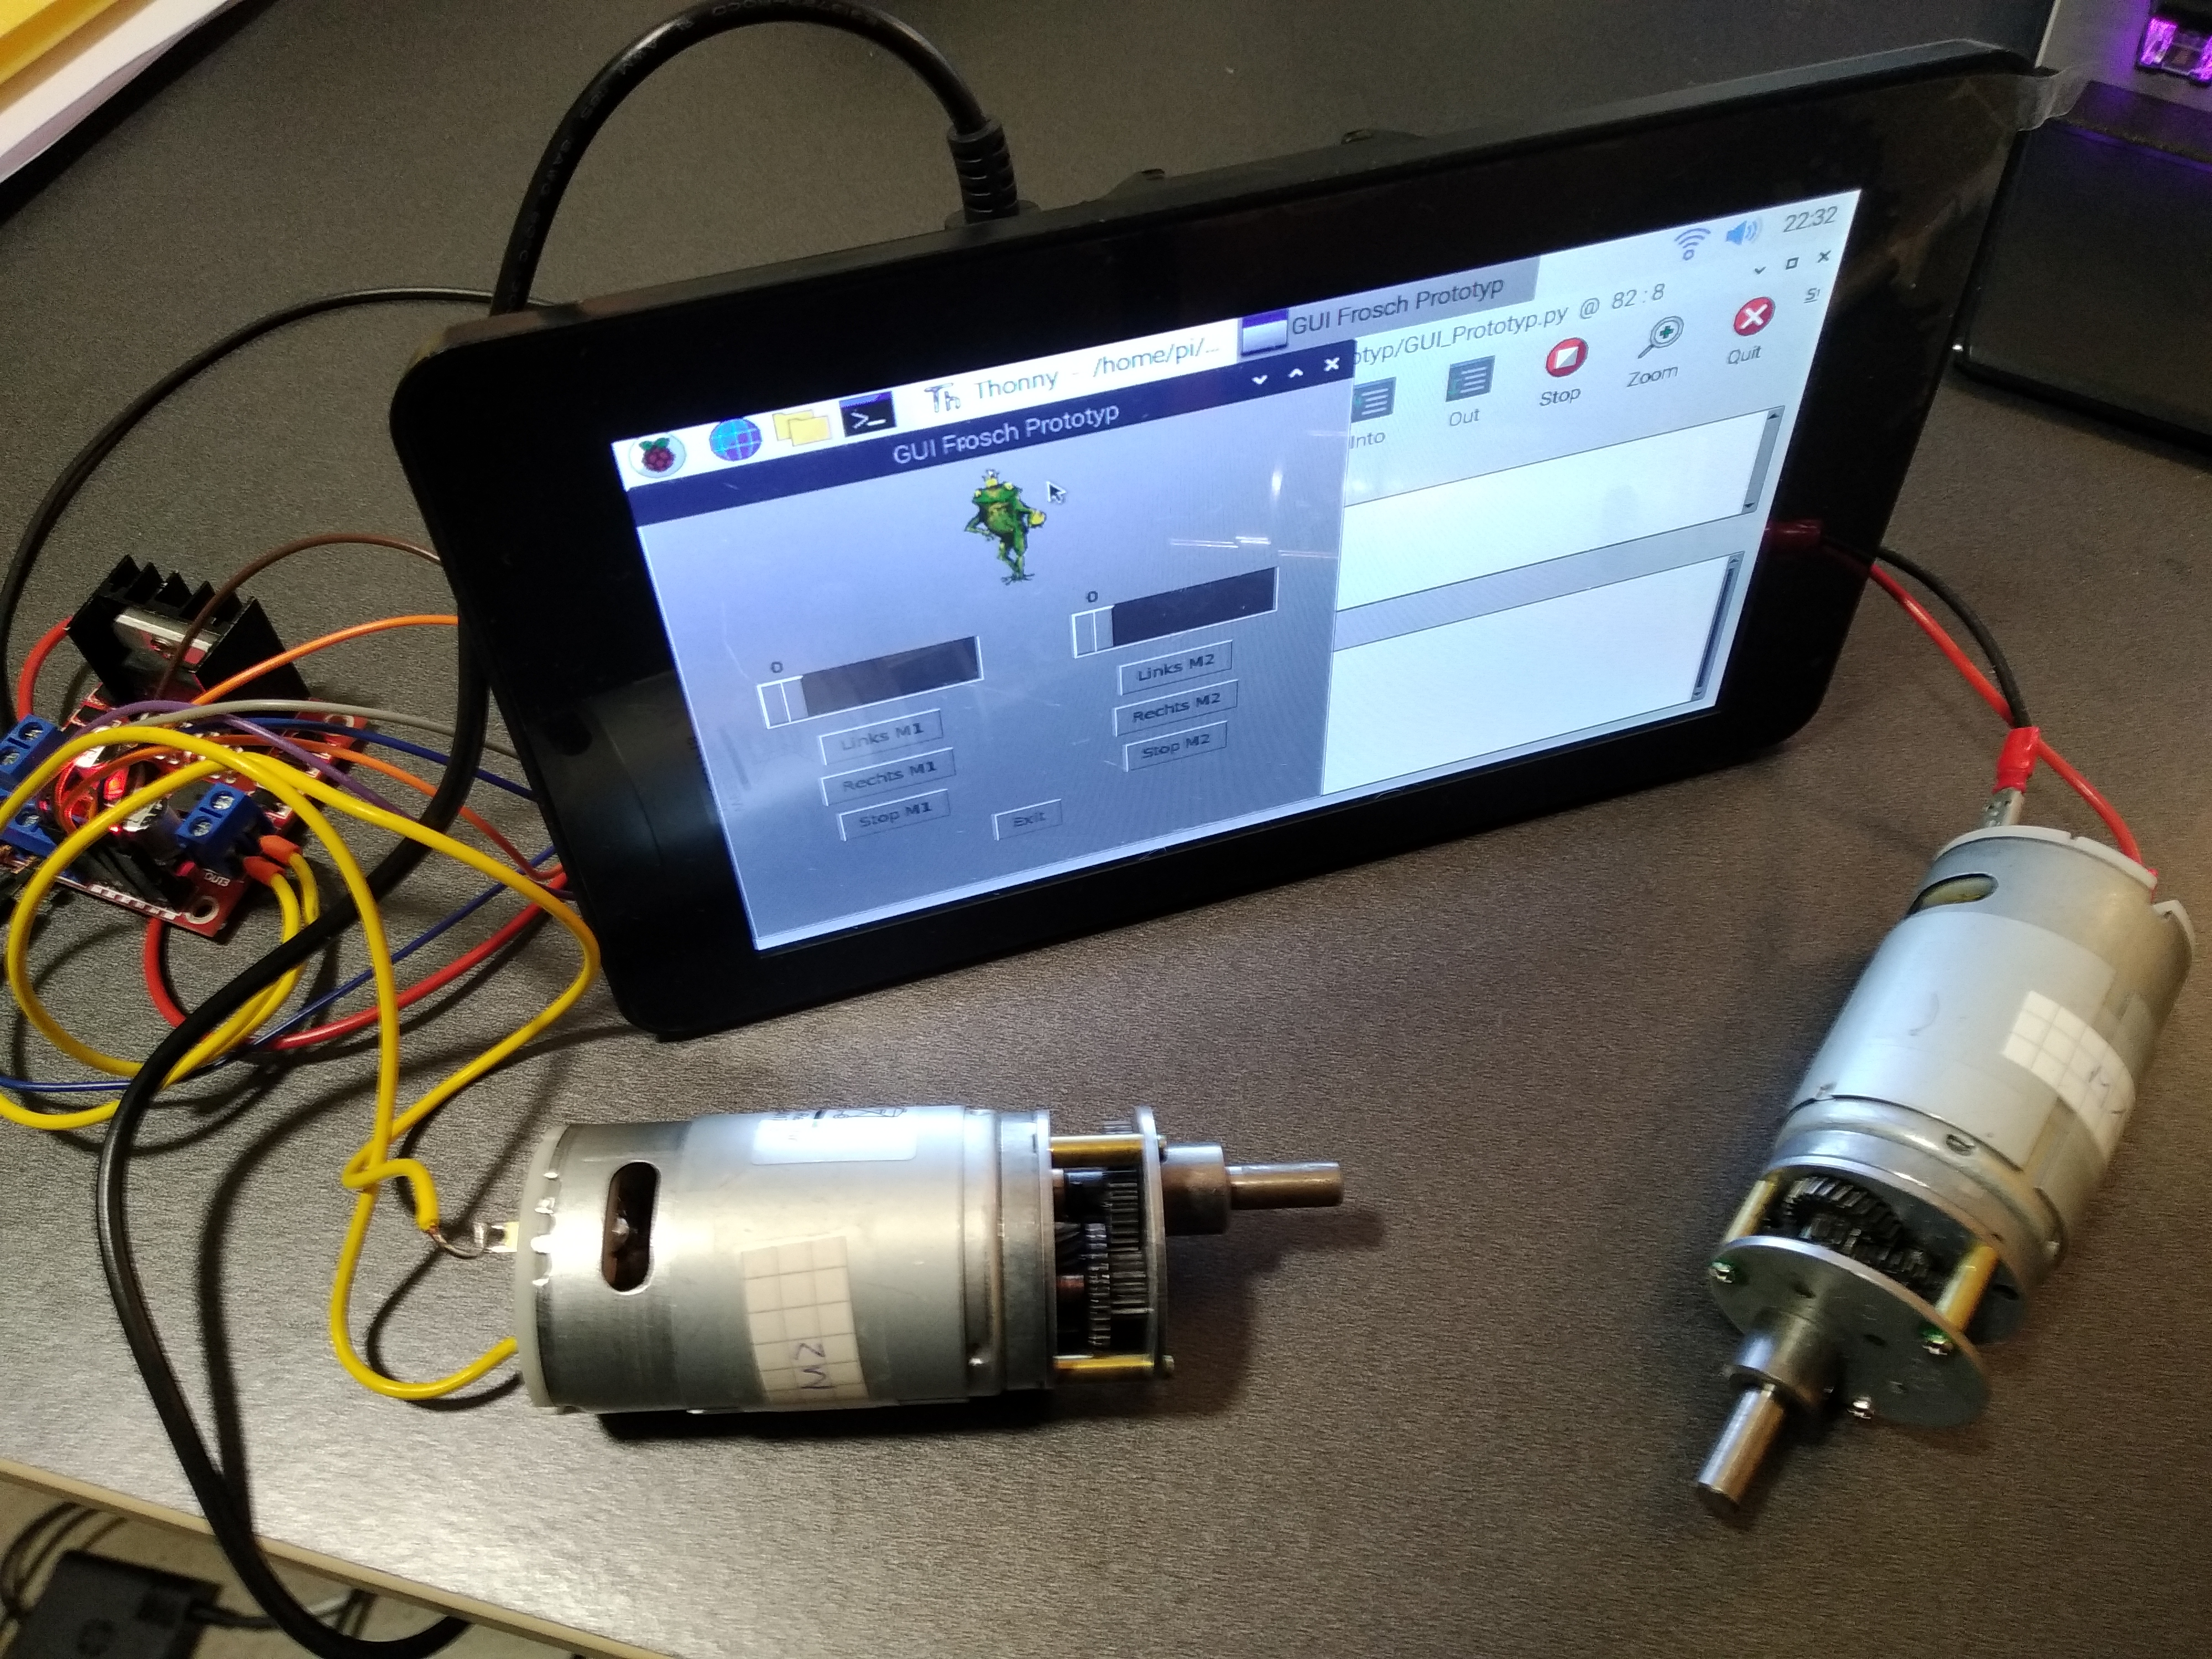
\includegraphics[width=0.6\textwidth]{img/Funktionsmuster Treppensteigen/Elektrische_Kompnenten.png}
  \centering
  \caption{Elektrische Komponenten des Prototyps}
\end{figure}

Um die Geschwindigkeit der Motoren individuell anpassen zu können, generiert der Raspberry Pi ein PWM-Signal für die H-Brücke. Dieses PWM-Signal kann in einem GUI mittels Slider von 0 bis 100\% verstellt werden. 
\newpage

\begin{figure}[h]
  \includegraphics[width=0.6\textwidth]{img/Funktionsmuster Treppensteigen/GUI_Prototyp.png}
  \centering
  \caption{GUI der Steuerung des Prototyps}
\end{figure}

Des Weiteren hat man die Möglichkeit auf dem GUI die Drehrichtung der einzelnen Motoren nach links und nach rechts zu wählen, sowie einzeln zu stoppen.

\subsubsection{Fazit}

Mit diesem Prototypen sollten die Hubbewegungen automatisiert werden. Dies ist so nicht gelungen, jedoch konnte mit dem Prototyp das Funktionsprinzip überprüft werden.

Nach den ersten ersten Tests wird klar, dass diese Methode funktioniert. Es gilt jedoch einige Faktoren besonders zu beachten. Die grösste Erkenntnis ist, dass die Hubbewegung mit zwei Motoren durchgeführt werden muss. Je ein Motor treibt eine Achse an, welche synchron beide Seiten antreibt. Diese Kraftübertragung wurde mithilfe des Prototypens getestet. 